%%%%%%%%%%%%%%%%%%%%%%%%%%%%%%%%%%%%%%%%%%%%%%%%%%%%%%%%%%%%%%%%%%%%%%%%%%%%%%%
%% SOCIOL 723 -- Social Statistics II
%% Week 3: Maximum Likelihood -- Theory
%% Wenhao Jiang, Duke University, Fall 2026
%%%%%%%%%%%%%%%%%%%%%%%%%%%%%%%%%%%%%%%%%%%%%%%%%%%%%%%%%%%%%%%%%%%%%%%%%%%%%%%

\documentclass[aspectratio=169,11pt,xcolor=dvipsnames]{beamer}
\mode<presentation>

%% ---- fonts: Latin Modern Roman (the LaTeX default), serif throughout -------
\usepackage[T1]{fontenc}
\usepackage{lmodern}
\usefonttheme{serif}
\renewcommand{\familydefault}{\rmdefault}

%% ---- packages --------------------------------------------------------------
\usepackage{amsmath,amsfonts,amssymb,bm}
\usepackage{graphicx}
\usepackage{booktabs}
\usepackage{tikz}
\usetikzlibrary{arrows.meta,positioning,calc}
\usepackage[english]{babel}

\newcommand{\srcp}[1]{{\scriptsize\color{gray}(#1)}}
\newcommand{\srct}[1]{#1}

\DeclareMathOperator*{\argminop}{arg\,min}
\DeclareMathOperator*{\argmaxop}{arg\,max}
%% \limits forces the subscript underneath even in inline math
\newcommand{\argmin}{\argminop\limits}
\newcommand{\argmax}{\argmaxop\limits}
\DeclareMathOperator{\Cov}{Cov}
\DeclareMathOperator{\Var}{Var}
\DeclareMathOperator{\trace}{tr}
\DeclareMathOperator{\rank}{rank}
\DeclareMathOperator{\plim}{plim}
\newcommand{\indep}{\perp\!\!\!\perp}

%% ---- notation conventions (course-wide) ------------------------------------
\newcommand{\E}{E}
\newcommand{\En}{\mathbb{E}_n}
\newcommand{\R}{\mathbb{R}}
\newcommand{\X}{\bm{X}}
\newcommand{\Y}{\bm{y}}
\newcommand{\Ix}{\bm{I}}
\newcommand{\zero}{\bm{0}}
\newcommand{\bhat}{\hat{\bm{\beta}}}
\newcommand{\dto}{\overset{d}{\longrightarrow}}
\newcommand{\pto}{\overset{p}{\longrightarrow}}
\newcommand{\lik}{\mathcal{L}}
\newcommand{\loglik}{\ell}
\newcommand{\Info}{\mathcal{I}}
\newcommand{\SE}{\mathrm{se}}

%% ---- theme -----------------------------------------------------------------
\usetheme{default}
%% thin single-line header: clickable section names, current one highlighted.
%% (miniframes is deliberately not used: one dot per slide wraps to 4 rows here)
\setbeamerfont{section in head/foot}{size=\tiny}
\setbeamertemplate{headline}{%
  \begin{beamercolorbox}[wd=\paperwidth,ht=2.4ex,dp=1.1ex,%
                         leftskip=.3cm,rightskip=.3cm]{section in head/foot}%
    \usebeamerfont{section in head/foot}%
    \insertsectionnavigationhorizontal{.94\paperwidth}{}{}%
  \end{beamercolorbox}%
}

\definecolor{dukeblue}{RGB}{1,33,105}
\definecolor{accent}{RGB}{200,78,0}
\definecolor{softgray}{RGB}{242,242,245}

\setbeamercolor{structure}{fg=dukeblue}
\setbeamercolor{frametitle}{fg=dukeblue,bg=white}
\setbeamercolor{section in head/foot}{fg=white,bg=dukeblue}
\setbeamercolor{section in head/foot shaded}{fg=white!50!dukeblue,bg=dukeblue}
\setbeamercolor{alerted text}{fg=accent}
\setbeamercolor{block title}{fg=white,bg=dukeblue}
\setbeamercolor{block body}{fg=black,bg=softgray}
\setbeamercolor{block title alerted}{fg=white,bg=accent}
\setbeamercolor{block body alerted}{fg=black,bg=softgray}

\setbeamertemplate{footline}[page number]
%% continued frames keep the SAME font size and spill onto a new slide
\setbeamertemplate{frametitle continuation}{\ifnum\insertcontinuationcount>1\normalfont\footnotesize\ (cont.)\fi}
\setbeamertemplate{navigation symbols}{}
\setbeamertemplate{itemize items}[circle]
\setbeamertemplate{blocks}[rounded][shadow=false]
\setbeamerfont{frametitle}{series=\bfseries}
\setbeamerfont{footnote}{size=\scriptsize}
\setbeamerfont{caption}{size=\footnotesize}
\setbeamertemplate{subsection in head/foot}{}
\setbeamertemplate{subsection in head/foot shaded}{}
\setbeamertemplate{caption}[numbered]

\newcommand{\adv}{\,\raisebox{0.6pt}{\textcolor{accent}{$\bigstar$}}}
%% marker for essential material every student must understand (examinable core)
\definecolor{corestar}{RGB}{0,83,155}
\newcommand{\core}{\,\raisebox{0.6pt}{\textcolor{corestar}{$\bigstar$}}}

\setbeamertemplate{section page}{%
  \begin{centering}\vfill
  {\usebeamercolor[fg]{structure}\Large\bfseries\insertsectionhead\par}
  \vskip4pt{\color{dukeblue}\rule{0.35\linewidth}{1pt}\par}
  \vfill\end{centering}}
\setbeamertemplate{subsection page}{%
  \begin{centering}\vfill
  {\usebeamercolor[fg]{structure}\large\bfseries\insertsubsectionhead\par}
  \vfill\end{centering}}

\AtBeginDocument{%
  \setlength{\abovedisplayskip}{5pt}%
  \setlength{\belowdisplayskip}{5pt}%
  \setlength{\abovedisplayshortskip}{2pt}%
  \setlength{\belowdisplayshortskip}{3pt}%
}
\setbeamertemplate{frametitle}{%
  \vskip4pt\usebeamerfont{frametitle}\usebeamercolor[fg]{frametitle}%
  \insertframetitle\par\vskip2pt}
\setbeamersize{text margin left=0.75cm, text margin right=0.75cm}

%% ---- title -----------------------------------------------------------------
%% ---- title page: same face as the body (Latin Modern), larger and bold
\setbeamerfont{title}{size*={16}{19},series=\bfseries}
\setbeamerfont{subtitle}{size=\Large,series=\mdseries}
\setbeamerfont{author}{size=\large}
\setbeamerfont{date}{size=\large}
\title[SOCIOL 723]{SOCIOL 723: Social Statistics II\\[-2pt]}
\subtitle{Week 3, Maximum Likelihood: Theory\\[-6pt]}
\author[Jiang]{Wenhao Jiang\vspace{-2.5em}}
\institute[Duke]{}
\titlegraphic{
\includegraphics[height=1.3cm]{../Misc/duke_logo.png}}
\date{Department of Sociology, Fall 2026}

\begin{document}

\begin{frame}[plain]
  \titlepage
\end{frame}

\begin{frame}{Today}
  \tableofcontents
  \vskip6pt
  {\footnotesize \core{} $=$ essential, you must understand this \quad\quad \adv{} $=$ for understanding, not examined}
\end{frame}

%%%%%%%%%%%%%%%%%%%%%%%%%%%%%%%%%%%%%%%%%%%%%%%%%%%%%%%%%%%%%%%%%%%%%%%%%%%%%%%
\section[Why Likelihood]{Why We Need More Than Least Squares}
%%%%%%%%%%%%%%%%%%%%%%%%%%%%%%%%%%%%%%%%%%%%%%%%%%%%%%%%%%%%%%%%%%%%%%%%%%%%%%%
\begin{frame}\sectionpage\end{frame}

\begin{frame}{What Least Squares Bought Us, and What It Cost\core}
Two weeks, one idea: pick the line that makes the squared misses as small as
possible. Look at how much that bought:
\begin{itemize}\itemsep3pt
  \item A slope with a clear meaning (the best linear approximation to the
        CEF), computable with sums alone.
  \item Honest uncertainty for it, robust to heteroskedasticity and
        clustering, without ever assuming what the errors look like.
\end{itemize}
\vskip2pt
It asked almost nothing in return: never \emph{how} $Y$ was generated,
only \emph{which line fits best}.
\vskip2pt
\begin{alertblock}{That is also its limit}
Least squares cannot ask \alert{how were these outcomes produced?} For
earnings you can afford not to ask. For much of sociology's data, you cannot.
\end{alertblock}
\end{frame}

\begin{frame}{Where the Line Runs Out\core}
Regress ``employed'' ($0/1$) on years of schooling, by least squares:
\vskip4pt
\begin{columns}[c]
\begin{column}{0.52\textwidth}
\centering
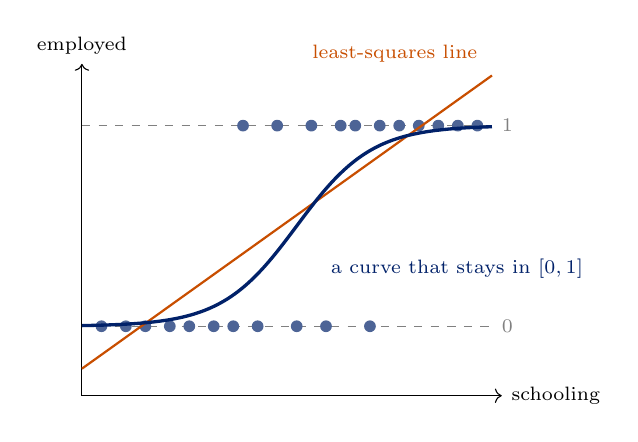
\begin{tikzpicture}[xscale=0.62,yscale=0.98]
  \draw[->] (0,-0.9) -- (8.6,-0.9) node[right]{\scriptsize schooling};
  \draw[->] (0,-0.9) -- (0,3.4) node[above]{\scriptsize employed};
  \draw[gray,dashed] (0,0) -- (8.4,0) node[right]{\scriptsize $0$};
  \draw[gray,dashed] (0,2.6) -- (8.4,2.6) node[right]{\scriptsize $1$};
  \foreach \x in {0.4,0.9,1.3,1.8,2.2,2.7,3.1,3.6,4.4,5.0,5.9}
    \node[circle,fill=dukeblue!70,inner sep=1.5pt] at (\x,0) {};
  \foreach \x in {3.3,4.0,4.7,5.3,5.6,6.1,6.5,6.9,7.3,7.7,8.1}
    \node[circle,fill=dukeblue!70,inner sep=1.5pt] at (\x,2.6) {};
  \draw[accent,thick] (0,-0.55) -- (8.4,3.25);
  \node[accent,anchor=south east] at (8.3,3.3) {\scriptsize least-squares line};
  \draw[dukeblue,very thick,smooth,samples=80,domain=0:8.4,variable=\x]
    plot ({\x},{2.6/(1+exp(-1.3*(\x-4.4)))});
  \node[dukeblue,anchor=west] at (4.9,0.75) {\scriptsize a curve that stays in $[0,1]$};
\end{tikzpicture}
\end{column}
\begin{column}{0.46\textwidth}
\begin{itemize}\itemsep6pt
  \item The line predicts ``probabilities'' below $0$ and above $1$: the
        shape of the outcome carries information the line cannot use.
  \item Counts go negative the same way; durations get censored;
        categories have no order. The problem is not the slope:
        \alert{a line is the wrong \emph{kind} of answer}.
\end{itemize}
\end{column}
\end{columns}
\end{frame}

\begin{frame}{The Question Underneath\core}
Least squares asks which line comes closest to the points. Maximum
likelihood asks something different:
\begin{center}
\alert{``Which parameter values would have made the data I observed most likely?''}
\end{center}
To ask that, you have to say how $Y$ is produced: a coin for employment, a
bell curve centred on a line for earnings. In return:
\begin{itemize}\itemsep2pt
  \item One method for any outcome: binary, count, ordered, duration.
  \item Standard errors from the shape of the likelihood, not a new formula
        per model.
  \item One way to test hypotheses, logit or Poisson alike: three tests
        read off the same curve.
  \item Nothing lost: with bell-shaped errors it returns the least-squares
        line exactly. (Call this \emph{the hook}; we cash it at the end of
        the next section.)
\end{itemize}
\vskip6pt
Hence two weeks: this week the method, next week logit, probit, Poisson.
\end{frame}

\begin{frame}{Two Stances, Both Legitimate}
Two questions, two stances toward a regression; this course uses both.
\begin{itemize}\itemsep4pt
  \item \textbf{Design-based} (Weeks 1--2, 5--11): $\beta$ is the best
        linear approximation to the CEF; assume little about how $Y$ was
        generated; let the \emph{research design} carry the causal claim.
  \item \textbf{Model-based} (Weeks 3--4): write a probability model for
        $Y$ and estimate the parameter values that make the data most
        probable. Needed when the outcome is not a continuous, unbounded number.
\end{itemize}
\vskip4pt
\begin{block}{Neither is ``the right one''}
Say which stance a result rests on: a logit coefficient and a
difference-in-differences estimate answer different kinds of question.
\end{block}
\end{frame}

%%%%%%%%%%%%%%%%%%%%%%%%%%%%%%%%%%%%%%%%%%%%%%%%%%%%%%%%%%%%%%%%%%%%%%%%%%%%%%%
\section[The Likelihood]{The Likelihood Function}
%%%%%%%%%%%%%%%%%%%%%%%%%%%%%%%%%%%%%%%%%%%%%%%%%%%%%%%%%%%%%%%%%%%%%%%%%%%%%%%
\begin{frame}\sectionpage\end{frame}

\begin{frame}{Probability Versus Likelihood\core}
Both start from the same object, the density (or mass function) $f(y\mid\theta)$.
What differs is \emph{what you hold fixed}.
\vskip2pt
\begin{columns}[T]
\begin{column}{0.47\textwidth}
\textbf{Probability}
\begin{align*}
  f(y\mid\theta)
\end{align*}
$\theta$ is \emph{fixed and known}; $y$ varies.\\[4pt]
``If the coin is fair, how likely am I to see 7 heads in 10 tosses?''
\end{column}
\begin{column}{0.49\textwidth}
\textbf{Likelihood}
\begin{align*}
  \lik(\theta;y) \equiv f(y\mid\theta)
\end{align*}
$y$ is \emph{fixed} (it is your data); $\theta$ varies.\\[4pt]
``Given that I saw 7 heads in 10 tosses, which values of $\theta$ make that
outcome most probable?''
\end{column}
\end{columns}
\vskip4pt
\begin{alertblock}{The single most important sentence today}
The likelihood is \emph{the same formula read backwards}: a function of
$\theta$ with the data fixed. It is \alert{not} a distribution over
$\theta$: it does not integrate to one.
\end{alertblock}
\end{frame}

\begin{frame}{A First Example: Marbles in a Bag\core}
An opaque bag holds blue and white marbles; $\theta$ is the proportion blue.
You draw 10 marbles \emph{with replacement} and get 7 blue. Ten draws are
ten \emph{observations}, each a Bernoulli outcome (blue or not); the
summary ``7 of 10'' is a binomial count. Build its probability step by step:
\begin{itemize}\itemsep2pt
  \item \textbf{One draw}: blue with probability $\theta$, white with
        probability $1-\theta$ (replacement makes the draws identical and
        independent).
  \item \textbf{One particular sequence}, say B\,B\,B\,B\,B\,B\,B\,W\,W\,W:
        independence means multiply,
        $\theta\cdot\theta\cdots\theta\cdot(1-\theta)(1-\theta)(1-\theta)
        = \theta^{7}(1-\theta)^{3}$. Any other order with 7 blues and 3
        whites has the \emph{same} product.
  \item \textbf{All such sequences}: there are
        $\binom{10}{3} = \binom{10}{7} = \frac{10!}{3!\,7!} = 120$ ways to
        place the 3 whites (equivalently the 7 blues) among the 10 draws,
        so $\Pr(7 \text{ blue} \mid \theta) = 120\,\theta^{7}(1-\theta)^{3}$.
        ($\binom{n}{k}$, read ``$n$ choose $k$,'' is the standard notation.)
\end{itemize}
The $120$ does not involve $\theta$: it cannot change which candidate wins.
\end{frame}

\begin{frame}{Marbles: Reading It as a Likelihood}
Now hold the data fixed, 7 blue in 10, and let $\theta$ vary:
\begin{align*}
  \lik(\theta) = 120\,\theta^{7}(1-\theta)^{3} .
\end{align*}
\begin{itemize}\itemsep3pt
  \item Try $\theta = 0.3$: $\lik = 120(0.3)^7(0.7)^3 \approx 0.0090$.
  \item Try $\theta = 0.5$: $\lik = 120(0.5)^{10} \approx 0.117$.
  \item Try $\theta = 0.7$: $\lik = 120(0.7)^7(0.3)^3 \approx 0.267$.
\end{itemize}
\vskip3pt
Among these three, $\theta = 0.7$ makes the data we actually saw most
probable. The MLE is the value that does best among \emph{all}
$\theta\in[0,1]$: the next frame plots the whole curve.
\end{frame}

\begin{frame}{The Likelihood, Plotted}
\begin{center}
\begin{tikzpicture}[scale=1]
  \draw[->] (0,0) -- (9.3,0) node[right]{\small $\theta$};
  \draw[->] (0,0) -- (0,3.4) node[above]{\small $\lik(\theta)$};
  \foreach \t/\lab in {0/0, 2/0.25, 4/0.5, 6/0.75, 8/1}
    \draw (\t,0) -- (\t,-0.08) node[below]{\scriptsize \lab};
  % binomial(10,7) likelihood, scaled: peak 0.2668 at 0.7 -> y=3
  \draw[dukeblue,very thick,smooth,samples=100,domain=0.02:0.98,variable=\x]
    plot ({8*\x},{3*120*(\x)^7*(1-\x)^3/0.26683});
  \draw[accent,dashed,thick] (5.6,0) -- (5.6,3);
  \node[accent] at (6.5,3.2) {\small $\hat\theta = 0.7$};
\end{tikzpicture}
\end{center}
\vskip-4pt
\begin{itemize}\itemsep2pt
  \item The height at any $\theta$ is the probability of \emph{these} data if that
        $\theta$ were true.
  \item The peak is the MLE. The \alert{width} of the peak will turn out to be our
        measure of uncertainty; that is the whole of Section 4.
\end{itemize}
\end{frame}

\begin{frame}{From One Observation to Many\core}
With $n$ observations we need the \emph{joint} density
$f(y_1,\dots,y_n\mid\theta)$. If the observations are independent given $\theta$,
it factors:
\begin{align*}
  \lik(\theta; y_1,\dots,y_n) = \prod_{i=1}^{n} f(y_i \mid \theta) .
\end{align*}
{\footnotesize (Two observations first: independence means
$f(y_1, y_2 \mid \theta) = f(y_1 \mid \theta)\, f(y_2 \mid \theta)$, the
probability of both is the product; $n$ observations just repeat the step.)}
\pause
A product of hundreds of numbers below one rounds to zero on a computer
and is awkward to differentiate, so we take logs:
\begin{align*}
  \boxed{\;\loglik(\theta) \equiv \log \lik(\theta) = \sum_{i=1}^{n}\log f(y_i\mid\theta)\;}
\end{align*}
\vskip2pt
\begin{itemize}\itemsep2pt
  \item $\log$ is strictly increasing, so it \alert{does not move the maximum}.
  \item A product becomes a sum, so the derivative is a sum over
        observations: setting it to zero is a kind of averaging.
\end{itemize}
\end{frame}

\begin{frame}{Worked Example 1: Bernoulli Draws\core}
The marble game: $n$ Bernoulli draws, $Y_i \in \{0,1\}$,
$\Pr(Y_i=1)=\theta$. We observe the $n$ draws and estimate $\theta$, the
probability of a success. One draw's mass function as a single formula:
\begin{align*}
  f(y_i\mid\theta) = \theta^{y_i}(1-\theta)^{1-y_i} .
\end{align*}
(At $y_i = 1$ it gives $\theta$; at $y_i = 0$, $1-\theta$.)
\begin{align*}
  \lik(\theta)
  &= \prod_{i=1}^n \theta^{y_i}(1-\theta)^{1-y_i}
   = \theta^{\sum_i y_i}(1-\theta)^{n - \sum_i y_i} , \\[1pt]
  \loglik(\theta)
  &= \Big(\textstyle\sum_i y_i\Big)\log\theta
   + \Big(n - \textstyle\sum_i y_i\Big)\log(1-\theta) .
\end{align*}
\textbf{Sequence or count?} This is the probability of the \emph{particular}
$0/1$ sequence; the binomial multiplies it by $\binom{n}{\sum y_i}$ for the
\emph{count}. A constant factor, so the same MLE: \alert{the total
$\sum_i y_i$ is all the data can tell you about $\theta$}.
\end{frame}

\begin{frame}{Worked Example 1: Reading the Binomial\core}
\begin{align*}
  \Pr(Y = y \mid n, \theta) = \binom{n}{y}\,\theta^{y}(1-\theta)^{n-y},
  \qquad y = 0, 1, \dots, n
\end{align*}
\vskip-4pt
\begin{center}
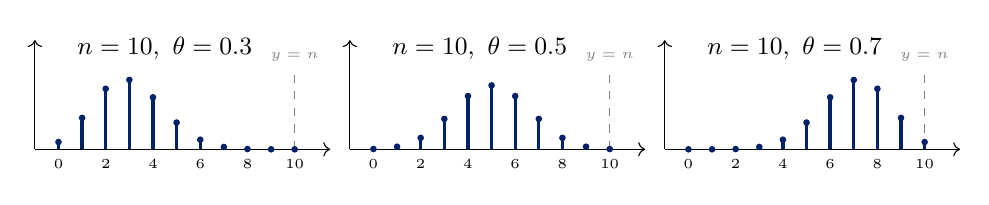
\begin{tikzpicture}[x=0.3cm,y=3.3cm]
  \begin{scope}[xshift=0.0cm]
    \draw[->] (-1,0) -- (11.5,0); \draw[->] (-1,0) -- (-1,0.42);
    \draw[gray,dashed] (10,0) -- (10,0.3); \node[gray,above] at (10,0.3) {\tiny $y=n$};
    \foreach \y/\p in {0/0.028,1/0.121,2/0.233,3/0.267,4/0.200,5/0.103,6/0.037,7/0.009,8/0.001,9/0.000,10/0.000}
      {\draw[dukeblue,very thick] (\y,0) -- (\y,\p); \fill[dukeblue] (\y,\p) circle (1.2pt);}
    \foreach \y in {0,2,4,6,8,10} \node[below] at (\y,0) {\tiny \y};
    \node at (4.5,0.39) {\small $n = 10,\ \theta = 0.3$};
  \end{scope}
  \begin{scope}[xshift=4.0cm]
    \draw[->] (-1,0) -- (11.5,0); \draw[->] (-1,0) -- (-1,0.42);
    \draw[gray,dashed] (10,0) -- (10,0.3); \node[gray,above] at (10,0.3) {\tiny $y=n$};
    \foreach \y/\p in {0/0.001,1/0.010,2/0.044,3/0.117,4/0.205,5/0.246,6/0.205,7/0.117,8/0.044,9/0.010,10/0.001}
      {\draw[dukeblue,very thick] (\y,0) -- (\y,\p); \fill[dukeblue] (\y,\p) circle (1.2pt);}
    \foreach \y in {0,2,4,6,8,10} \node[below] at (\y,0) {\tiny \y};
    \node at (4.5,0.39) {\small $n = 10,\ \theta = 0.5$};
  \end{scope}
  \begin{scope}[xshift=8.0cm]
    \draw[->] (-1,0) -- (11.5,0); \draw[->] (-1,0) -- (-1,0.42);
    \draw[gray,dashed] (10,0) -- (10,0.3); \node[gray,above] at (10,0.3) {\tiny $y=n$};
    \foreach \y/\p in {0/0.000,1/0.000,2/0.001,3/0.009,4/0.037,5/0.103,6/0.200,7/0.267,8/0.233,9/0.121,10/0.028}
      {\draw[dukeblue,very thick] (\y,0) -- (\y,\p); \fill[dukeblue] (\y,\p) circle (1.2pt);}
    \foreach \y in {0,2,4,6,8,10} \node[below] at (\y,0) {\tiny \y};
    \node at (4.5,0.39) {\small $n = 10,\ \theta = 0.7$};
  \end{scope}
\end{tikzpicture}
\end{center}
\vskip-4pt
\begin{itemize}\itemsep2pt
  \item \textbf{The pieces}: $\theta^{y}$ for the $y$ successes,
        $(1-\theta)^{n-y}$ for the failures, $\binom{n}{y}$ for the orders
        they can come in.
  \item \textbf{The shape}: mean $n\theta$, variance $n\theta(1-\theta)$
        ($n$ independent draws with mean $\theta$ and variance
        $\theta(1-\theta)$; both add), and a hard ceiling at $n$.
  \item \textbf{Fix the data, compare the panels}: fix $y = 7$; which
        panel puts the most mass on $7$? The $\theta = 0.7$ panel. Data
        fixed, $\theta$ varying: the likelihood.
\end{itemize}
\end{frame}

\begin{frame}{Counting Units or Counting Events?\core}
Sociology's counts come in two kinds.
\begin{itemize}\itemsep5pt
  \item \textbf{Units with an event, out of a known $n$}: 12 of 30 students
        protested. Each unit is a Bernoulli $0/1$ (Worked Example 1); the
        total is binomial; it cannot exceed $n$.
  \item \textbf{Events one unit accumulates over exposure}: arrests of one
        person in a year; children; publications. There is no $n$ to count
        out of, and no ceiling.
\end{itemize}
\vskip6pt
\begin{block}{Rule of thumb}
First kind: binomial (in practice a logit on the $0/1$, Week 4). Second
kind: we need a distribution with no ceiling. Build it from the binomial,
next.
\end{block}
\end{frame}

\begin{frame}{Worked Example 2: From the Binomial to the Poisson\core}
Start from the binomial count of Worked Example 1:
\begingroup\setlength{\abovedisplayskip}{2pt}\setlength{\belowdisplayskip}{2pt}
\begin{align*}
  \Pr(Y = y \mid n, p) = \binom{n}{y}\,p^{y}\,(1-p)^{n-y} .
\end{align*}
\endgroup
Read it as \emph{arrests of one person in a year}: slice the year into $n$
moments, each a Bernoulli trial with chance $p$ of an arrest. Then $y$ is
the number of arrests: $p^{y}$ for the $y$ moments with one, $(1-p)^{n-y}$
for the rest, $\binom{n}{y}$ for which moments they were.
\vskip2pt
Now slice finer: 365 days, 8{,}760 hours, 525{,}600 minutes, $\dots$ The
slices $n \to \infty$ and the chance per slice $p \to 0$, but the expected
arrests per year, $np = \E[Y] = \theta$, cannot depend on the slicing. Fix
$y$ and take the limit:
\begingroup\setlength{\abovedisplayskip}{2pt}\setlength{\belowdisplayskip}{2pt}
\begin{align*}
  \binom{n}{y}p^{y}(1-p)^{n-y} \ \longrightarrow\
  \frac{\theta^{y}e^{-\theta}}{y!}, \qquad y = 0, 1, 2, \dots
\end{align*}
\endgroup
The \alert{Poisson distribution}: one parameter $\theta$ (the letter is
recycled; it always means ``the parameter''), the expected count. Neither
$n$ nor $p$ survives, so nothing caps the count.
\vskip-3pt
{\footnotesize Why\adv: $p = \theta/n$, so $\binom{n}{y}p^{y} \to \theta^{y}/y!$
and $(1-\theta/n)^{n-y} \to e^{-\theta}$.}
\end{frame}

\begin{frame}{Worked Example 2: Reading the Poisson\core}
\begin{align*}
  \Pr(Y = y \mid \theta) = \frac{\theta^{y}\, e^{-\theta}}{y!},
  \qquad y = 0, 1, 2, \dots
\end{align*}
\vskip-4pt
\begin{center}
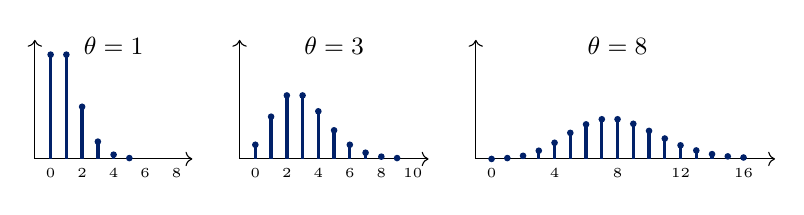
\begin{tikzpicture}[x=0.2cm,y=3.6cm]
  \begin{scope}
    \draw[->] (-1,0) -- (9,0); \draw[->] (-1,0) -- (-1,0.42);
    \foreach \y/\p in {0/0.368,1/0.368,2/0.184,3/0.061,4/0.015,5/0.003}
      {\draw[dukeblue,very thick] (\y,0) -- (\y,\p); \fill[dukeblue] (\y,\p) circle (1.2pt);}
    \foreach \y in {0,2,4,6,8} \node[below] at (\y,0) {\tiny \y};
    \node at (4,0.40) {\small $\theta = 1$};
  \end{scope}
  \begin{scope}[xshift=2.6cm]
    \draw[->] (-1,0) -- (11,0); \draw[->] (-1,0) -- (-1,0.42);
    \foreach \y/\p in {0/0.050,1/0.149,2/0.224,3/0.224,4/0.168,5/0.101,6/0.050,7/0.022,8/0.008,9/0.003}
      {\draw[dukeblue,very thick] (\y,0) -- (\y,\p); \fill[dukeblue] (\y,\p) circle (1.2pt);}
    \foreach \y in {0,2,4,6,8,10} \node[below] at (\y,0) {\tiny \y};
    \node at (5,0.40) {\small $\theta = 3$};
  \end{scope}
  \begin{scope}[xshift=5.6cm]
    \draw[->] (-1,0) -- (18,0); \draw[->] (-1,0) -- (-1,0.42);
    \foreach \y/\p in {0/0.000,1/0.003,2/0.011,3/0.029,4/0.057,5/0.092,6/0.122,7/0.140,8/0.140,9/0.124,10/0.099,11/0.072,12/0.048,13/0.030,14/0.017,15/0.009,16/0.005}
      {\draw[dukeblue,very thick] (\y,0) -- (\y,\p); \fill[dukeblue] (\y,\p) circle (1.2pt);}
    \foreach \y in {0,4,8,12,16} \node[below] at (\y,0) {\tiny \y};
    \node at (8,0.40) {\small $\theta = 8$};
  \end{scope}
\end{tikzpicture}
\end{center}
\vskip-4pt
\begin{itemize}\itemsep2pt
  \item \textbf{The pieces}: $\theta^y$ grows with $y$, $y!$ shrinks it back
        (large counts are rare), $e^{-\theta}$ makes the probabilities sum
        to one.
  \item \textbf{The shapes}: piled at zero and right-skewed for small
        $\theta$; nearly a bell centred at $\theta$ for large $\theta$. No
        ceiling anywhere: the binomial's $n$ is gone.
  \item \textbf{The signature}: mean and variance are both $\theta$
        (inherited from the binomial: $np \to \theta$ and
        $np(1-p) \to \theta$ as $p \to 0$). Spread grows with the mean.
\end{itemize}
\end{frame}

\begin{frame}{Worked Example 2: The Poisson Log-Likelihood\core}
Independent Poisson counts $Y_1,\dots,Y_n$, common $\theta$; step by step:
\begingroup
\setlength{\abovedisplayskip}{2pt}\setlength{\belowdisplayskip}{2pt}
\begin{align*}
  \lik(\theta) &= \prod_{i=1}^n \frac{\theta^{y_i}e^{-\theta}}{y_i!}
    && \text{\footnotesize independence: multiply} \\
  \loglik(\theta) &= \sum_{i=1}^n \log\!\left(\frac{\theta^{y_i}e^{-\theta}}{y_i!}\right)
    && \text{\footnotesize log turns the product into a sum} \\
  &= \sum_{i=1}^n \Big( y_i\log\theta - \theta - \log(y_i!)\Big)
    && \text{\footnotesize $\log\theta^{y} = y\log\theta$, $\log e^{-\theta} = -\theta$} \\
  &= \log(\theta)\sum_{i} y_i \;-\; n\theta \;-\; \sum_i \log(y_i!)
    && \text{\footnotesize collect: $n$ copies of $\theta$}
\end{align*}
\endgroup
\begin{itemize}\itemsep1pt
  \item The last term has no $\theta$: an \emph{additive constant},
        droppable for maximization but not when comparing log-likelihood
        \emph{values} across models.
  \item Again the data enter only through $\sum_i y_i$: the total count is
        sufficient.
\end{itemize}
\vskip-3pt
\end{frame}

\begin{frame}{Worked Example 3: The Normal Linear Model\core}
The normal (Gaussian) density, a bell centred at $\mu$ with spread $\sigma$:
\begin{align*}
  f(y \mid \mu, \sigma^2)
  = \frac{1}{\sqrt{2\pi\sigma^2}}\exp\!\left(-\frac{(y-\mu)^2}{2\sigma^2}\right) .
\end{align*}
One assumption from Week 1 and one new one, with $\sigma^2$ held fixed:
\begin{enumerate}\itemsep3pt
  \item \textbf{Linear CEF}: $\E[Y_i \mid X_i] = \beta_0 + \beta_1 X_i$.
  \item \textbf{Normal errors}: $\epsilon_i \sim \mathcal N(0,\sigma^2)$,
        independently.
\end{enumerate}
Together they say $Y_i \mid X_i \sim \mathcal N(\beta_0 + \beta_1 X_i,\
\sigma^2)$: the bell's centre $\mu$ is the line. Put $\mu = b_0 + b_1X_i$
into the density, and one observation's likelihood at candidate values
$(b_0,b_1)$ is
\begin{align*}
  f(Y_i \mid b_0, b_1)
  = \frac{1}{\sqrt{2\pi\sigma^2}}
    \exp\!\left(-\frac{(Y_i - b_0 - b_1 X_i)^2}{2\sigma^2}\right) .
\end{align*}
\end{frame}

\begin{frame}{Cashing the Hook: OLS Is an MLE\core}
Product over independent observations, then log:
\begin{align*}
  \loglik(b_0, b_1)
  &= \sum_{i=1}^n \log f(Y_i \mid b_0, b_1)
   = \sum_{i=1}^n \Big[ -\tfrac12\log(2\pi\sigma^2)
     - \frac{(Y_i - b_0 - b_1X_i)^2}{2\sigma^2} \Big] \\[1pt]
  &= \underbrace{-\frac n2\log(2\pi\sigma^2)}_{\text{no } b_0, b_1}
     \;-\; \frac{1}{2\sigma^2}
     \underbrace{\sum_{i=1}^n (Y_i - b_0 - b_1X_i)^2}_{\text{Week 1's } S(b_0,b_1)} .
\end{align*}
\begin{itemize}\itemsep2pt
  \item The candidates enter only through $S$, with a minus sign and a
        positive factor in front. \alert{Maximizing $\loglik$ is exactly
        minimizing $S$}: the MLE is the least-squares line, digit for digit.
  \item Least squares was never arbitrary: it is what ``make the data as
        probable as possible'' prescribes for normal errors around a line.
\end{itemize}
\end{frame}

\begin{frame}{What the Hook Does Not Say\core}
\begin{itemize}\itemsep6pt
  \item \textbf{OLS itself never needed normality.} Weeks 1--2 built it
        from moments alone; its large-sample inference came from the CLT.
        Normality entered only to make the $t$ table exact.
  \item \textbf{Normality is the price of admission} to the likelihood
        framework. For a continuous outcome it buys little: OLS already
        gave the estimate, and Week 2 already gave its standard errors.
\end{itemize}
\vskip6pt
\begin{block}{The point of the exercise}
Not ``assume normality,'' but ``one principle contains least squares as a
special case and extends to everything least squares cannot do.''
\end{block}
\end{frame}

\begin{frame}{Preview: Where the Regressors Go\core}
So far every observation shares one $\theta$. Next week each observation
gets its own, driven by covariates:
\begin{align*}
  \theta_i = \exp(\beta_0 + \beta_1 X_i),
  \qquad
  \loglik(\beta_0,\beta_1) = \sum_i \Big[\, y_i(\beta_0 + \beta_1 X_i)
  - e^{\beta_0 + \beta_1 X_i} - \log(y_i!)\Big] .
\end{align*}
\begin{itemize}\itemsep3pt
  \item The exponential keeps every $\theta_i$ positive, whatever the
        covariates do; this is the \emph{log link} of Poisson regression.
  \item Same recipe: density, product, log, sum. Only the parameter changed
        from a number to a function of $X_i$.
  \item No closed form any more ($\beta$ sits inside the exponential), so
        the maximum is found numerically: Section 3 does it by hand.
\end{itemize}
\end{frame}

%%%%%%%%%%%%%%%%%%%%%%%%%%%%%%%%%%%%%%%%%%%%%%%%%%%%%%%%%%%%%%%%%%%%%%%%%%%%%%%
\section[Finding the MLE]{Finding the Maximum}
%%%%%%%%%%%%%%%%%%%%%%%%%%%%%%%%%%%%%%%%%%%%%%%%%%%%%%%%%%%%%%%%%%%%%%%%%%%%%%%
\begin{frame}\sectionpage\end{frame}

\begin{frame}{The Score Function\core}
\begin{block}{Definition}
The \alert{score} is the derivative of the log-likelihood with respect to the
parameter:
\begin{align*}
  S(\theta) \;\equiv\; \frac{\partial \loglik(\theta)}{\partial\theta}
  \;=\; \sum_{i=1}^{n} \frac{\partial \log f(y_i\mid\theta)}{\partial \theta} .
\end{align*}
\end{block}
\vskip4pt
\begin{itemize}\itemsep3pt
  \item The MLE $\hat\theta$ solves $S(\hat\theta) = 0$, the
        \alert{first-order condition}, exactly as the normal equations were the
        FOC for least squares.
  \item Second-order condition: $\partial^2\loglik/\partial\theta^2 < 0$ at
        $\hat\theta$, so that we have a maximum rather than a minimum.
  \item Write $\theta_0$ for the \emph{true} value. A population fact,
        derived in Section 4: across repeated samples, $\E[S(\theta_0)] = 0$
        (the true $\theta_0$ fixed, the data varying: Week 2's
        sampling-distribution view).
\end{itemize}
\end{frame}

\begin{frame}{Bernoulli: Deriving $\hat\theta$\core}
\begin{align*}
  \loglik(\theta) &= \Big(\textstyle\sum_i y_i\Big)\log\theta
   + \Big(n - \textstyle\sum_i y_i\Big)\log(1-\theta) \\[4pt]
  S(\theta) &= \frac{\sum_i y_i}{\theta} - \frac{n - \sum_i y_i}{1-\theta}
  \ \overset{!}{=}\ 0 .
\end{align*}
\pause
Multiply through by $\theta(1-\theta)$:
\begin{align*}
  (1-\theta)\sum_i y_i - \theta\Big(n - \sum_i y_i\Big) &= 0 \\
  \sum_i y_i - \theta\sum_i y_i - n\theta + \theta\sum_i y_i &= 0 \\
  \boxed{\;\hat\theta = \frac{1}{n}\sum_i y_i = \bar y\;}
\end{align*}
The MLE of a probability is the sample proportion, derived, not assumed.
\end{frame}

\begin{frame}{Poisson: Deriving $\hat\theta$\core}
Differentiate the log-likelihood and set the score to zero:
\begin{align*}
  \loglik(\theta) &= \log(\theta)\sum_i y_i - n\theta - \sum_i\log(y_i!) \\[2pt]
  S(\theta) &= \frac{\sum_i y_i}{\theta} - n
    && \text{\footnotesize $\tfrac{d}{d\theta}\log\theta = \tfrac1\theta$;
       the constant's derivative is $0$} \\[2pt]
  S(\hat\theta) = 0 &\ \Longrightarrow\ \frac{\sum_i y_i}{\hat\theta} = n
   \ \Longrightarrow\ \boxed{\;\hat\theta = \frac{\sum_i y_i}{n} = \bar y\;}
\end{align*}
\vskip2pt
Second-order condition, to be sure it is a maximum:
\begin{align*}
  \frac{\partial^2 \loglik}{\partial\theta^2} = -\frac{\sum_i y_i}{\theta^2} < 0 .
  \quad\checkmark
\end{align*}
\vskip2pt
Both examples give $\bar y$, which is not a coincidence: for these
distributions the mean \emph{is} the parameter, and maximum likelihood
finds it.
\end{frame}

\begin{frame}{Normal Linear Model: Deriving $\hat\beta$ and $\hat\sigma^2$\core}
Three parameters, so three first-order conditions. With
$e_i = Y_i - b_0 - b_1X_i$:
\begingroup\small
\setlength{\abovedisplayskip}{2pt}\setlength{\belowdisplayskip}{2pt}
\begin{align*}
  \frac{\partial\loglik}{\partial b_0}
  &= \frac{1}{\sigma^2}\sum_i e_i \overset{!}{=} 0,
  \qquad
  \frac{\partial\loglik}{\partial b_1}
  = \frac{1}{\sigma^2}\sum_i X_i\, e_i \overset{!}{=} 0
    && \text{\footnotesize Week 1's normal equations, exactly} \\[4pt]
  \frac{\partial\loglik}{\partial\sigma^2}
  &= -\frac{n}{2\sigma^2} + \frac{1}{2\sigma^4}\sum_i e_i^2 \overset{!}{=} 0
  \quad\Longrightarrow\quad
  \hat\sigma^2 = \frac1n\sum_i \hat e_i^{\,2}
    && \text{\footnotesize solve; $\hat e_i$ are the OLS residuals}
\end{align*}
\endgroup
The first two conditions are Week 1's normal equations, so
$\hat\beta_0, \hat\beta_1$ are the OLS estimates: the hook, cashed a second
way.
\vskip3pt
\begin{alertblock}{The MLE of $\sigma^2$ is biased}
It divides by $n$, not $n-2$: $\E[\hat\sigma^2] = \frac{n-2}{n}\sigma^2 <
\sigma^2$. Week 1's $s^2$ was the bias-corrected version.
\end{alertblock}
\end{frame}

\begin{frame}{When There Is No Closed Form}
Most likelihoods you will meet, logit, probit, negative binomial, anything
with covariates, have no algebraic solution to $S(\theta)=0$. We search
numerically.
\vskip4pt
\begin{block}{Newton--Raphson}
Start at a guess $\theta^{[0]}$ (superscript in brackets: an iteration count, not the true value) and iterate
\begin{align*}
  \theta^{[t+1]} = \theta^{[t]} - \left[\frac{\partial^2\loglik}{\partial\theta^2}
  \bigg|_{\theta^{[t]}}\right]^{-1} S(\theta^{[t]}) ,
\end{align*}
a step of size score over curvature. The next frame draws it.
\end{block}
\vskip3pt
Variants: \textbf{BFGS} approximates the second derivative; \textbf{Fisher
scoring} uses its expectation (what \texttt{glm()} does).
\end{frame}

\begin{frame}{Finding the Peak: Newton--Raphson in a Picture}
\begin{center}
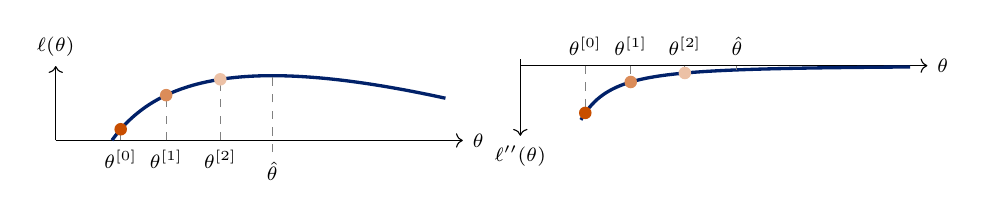
\begin{tikzpicture}[x=0.55cm,y=0.27cm]
  % Poisson, y = 5: l(theta) = 5 ln theta - theta; S = 5/theta - 1; l'' = -5/theta^2
  % Newton from 1.5: 1.5 -> 2.55 -> 3.80 -> 4.71 -> 5
  % ---------- left: the log-likelihood and the guesses ----------
  \begin{scope}
    \draw[->] (0,0) -- (9.4,0) node[right]{\scriptsize $\theta$};
    \draw[->] (0,0) -- (0,3.5) node[above]{\scriptsize $\loglik(\theta)$};
    \draw[dukeblue,very thick,smooth,samples=120,domain=1.3:9,variable=\x]
      plot ({\x},{5*ln(\x)-\x});
    \foreach \x/\lab in {1.5/{$\theta^{[0]}$},2.55/{$\theta^{[1]}$},3.8/{$\theta^{[2]}$}}
      {\draw[gray,dashed] (\x,0) -- (\x,{5*ln(\x)-\x});
       \node[below] at (\x,0) {\scriptsize \lab};}
    \draw[gray,dashed] (5,-0.55) -- (5,3.047); \node[below] at (5,-0.55) {\scriptsize $\hat\theta$};
    \node[circle,fill=accent,inner sep=1.6pt] at (1.5,0.527) {};
    \node[circle,fill=accent!65,inner sep=1.6pt] at (2.55,2.13) {};
    \node[circle,fill=accent!35,inner sep=1.6pt] at (3.8,2.875) {};
  \end{scope}
  % ---------- right: the second derivative, one curve ----------
  \begin{scope}[xshift=5.9cm,yshift=0.95cm]
    \draw[->] (0,0) -- (9.4,0) node[right]{\scriptsize $\theta$};
    \draw[->] (0,0.3) -- (0,-3.3) node[below]{\scriptsize $\loglik''(\theta)$};
    \draw[dukeblue,very thick,smooth,samples=120,domain=1.4:9,variable=\x]
      plot ({\x},{-5/(\x*\x)});
    \foreach \x/\lab in {1.5/{$\theta^{[0]}$},2.55/{$\theta^{[1]}$},3.8/{$\theta^{[2]}$},5/{$\hat\theta$}}
      {\draw[gray,dashed] (\x,0) -- (\x,{-5/(\x*\x)});
       \node[above] at (\x,0) {\scriptsize \lab};}
    \node[circle,fill=accent,inner sep=1.6pt] at (1.5,-2.222) {};
    \node[circle,fill=accent!65,inner sep=1.6pt] at (2.55,-0.769) {};
    \node[circle,fill=accent!35,inner sep=1.6pt] at (3.8,-0.346) {};
  \end{scope}
\end{tikzpicture}
\end{center}
\vskip-8pt
\begin{center}\scriptsize
\renewcommand{\arraystretch}{1.0}
\begin{tabular}{lcccc}
\toprule
guess $\theta$ & 1.50 & 2.55 & 3.80 & 4.71 \\
slope $S$ & 2.33 & 0.96 & 0.32 & 0.06 \\
$-\loglik''$ & 2.22 & 0.77 & 0.35 & 0.23 \\
step $S/(-\loglik'')$ & 1.05 & 1.25 & 0.91 & 0.27 \\
\bottomrule
\end{tabular}
\end{center}
\vskip-1pt
\begin{itemize}\itemsep0pt
  \item Poisson, one observation $y = 5$: $\loglik = 5\log\theta - \theta$,
        right panel $\loglik'' = -5/\theta^{2}$. Step $=$ slope
        $\div (-\loglik'')$: gradient ascent with the step set by the curvature.
  \item The step is a \emph{ratio} of two things that both change with
        $\theta$; it stops when the slope is zero. $-\loglik''(\hat\theta)$
        is the observed information: next section.
\end{itemize}
\end{frame}

\begin{frame}{Poisson by Hand: Newton--Raphson\core}
Five counts: $2, 0, 3, 1, 4$. So $n = 5$, $\sum y_i = 10$, and we know the
answer, $\hat\theta = \bar y = 2$. Pretend we do not.
\begingroup\setlength{\abovedisplayskip}{2pt}\setlength{\belowdisplayskip}{2pt}
\begin{align*}
  \loglik(\theta) = 10\log\theta - 5\theta + \text{const},
  \qquad
  S(\theta) = \frac{10}{\theta} - 5,
  \qquad
  \loglik''(\theta) = -\frac{10}{\theta^{2}} .
\end{align*}
\endgroup
Start at a guess $\theta^{[0]} = 1$ and step by slope over curvature,
$\theta^{[t+1]} = \theta^{[t]} - S/\loglik''$:
\begin{center}
\renewcommand{\arraystretch}{1.1}
\begin{tabular}{ccccc}
\toprule
guess $\theta$ & slope $S$ & $-\loglik''$ & step $S/(-\loglik'')$ & next guess \\
\midrule
1.000 & 5.000 & 10.00 & 0.500 & 1.500 \\
1.500 & 1.667 & 4.44  & 0.375 & 1.875 \\
1.875 & 0.333 & 2.84  & 0.117 & 1.992 \\
1.992 & 0.020 & 2.52  & 0.008 & 2.000 \\
\bottomrule
\end{tabular}
\end{center}
\vskip2pt
Four steps to $2.000$. At the answer $S = 0$ and $-\loglik''(2) = 2.5$: the
observed information, so $\SE = 1/\sqrt{2.5} = 0.63$. Check:
$\sqrt{\bar y/n} = \sqrt{2/5} = 0.63$.
\end{frame}

\begin{frame}{Regressors Inside: $\beta_1$ by Hand, the Function\core}
Give each count its own mean, $\theta_i = e^{\beta_1 X_i}$ (intercept known
to be $0$ for now). Four made-up observations, $X = 0, 1, 2, 3$ and
$y = 1, 2, 4, 8$. The Poisson log-likelihood is
$\sum_i [\, y_i \log\theta_i - \theta_i\,]$ plus a constant, and
$\log\theta_i = \beta_1 X_i$. Write out all four terms:
\begingroup\small\setlength{\abovedisplayskip}{2pt}\setlength{\belowdisplayskip}{2pt}
\begin{align*}
  \loglik(\beta_1)
  &= \big[1\cdot\beta_1\cdot 0 - e^{0}\big]
   + \big[2\cdot\beta_1\cdot 1 - e^{\beta_1}\big]
    && \text{\footnotesize $i = 1, 2$: $X_i = 0, 1$; $y_i = 1, 2$} \\
  &\quad + \big[4\cdot\beta_1\cdot 2 - e^{2\beta_1}\big]
   + \big[8\cdot\beta_1\cdot 3 - e^{3\beta_1}\big]
    && \text{\footnotesize $i = 3, 4$: $X_i = 2, 3$; $y_i = 4, 8$} \\
  &= 34\,\beta_1 \;-\; 1 - e^{\beta_1} - e^{2\beta_1} - e^{3\beta_1}
    && \text{\footnotesize $0 + 2 + 8 + 24 = 34$} \\[3pt]
  S(\beta_1) &= 34 \;-\; e^{\beta_1} - 2e^{2\beta_1} - 3e^{3\beta_1}
    && \text{\footnotesize differentiate: $\tfrac{d}{d\beta_1}e^{kX\beta_1} = k\,e^{k\beta_1}$} \\[3pt]
  \loglik''(\beta_1) &= -\,e^{\beta_1} - 4e^{2\beta_1} - 9e^{3\beta_1}
    && \text{\footnotesize differentiate again; always negative}
\end{align*}
\endgroup
\vskip2pt
$S(\beta_1) = 0$ has no closed form: $\beta_1$ sits inside three different
exponentials. But try $\beta_1 = \log 2$, so $e^{\beta_1} = 2$:
$S = 34 - 2 - 2\cdot 4 - 3\cdot 8 = 0$. That is the answer; Newton finds it
without the lucky guess.
\end{frame}

\begin{frame}{Regressors Inside: $\beta_1$ by Hand, the Iterations\core}
Slope over curvature, starting from $\beta_1 = 0.5$. At each guess, first the
four fitted means $\theta_i = e^{\beta_1 X_i}$, then $S$ and $\loglik''$
from the previous frame:
\begin{center}
\renewcommand{\arraystretch}{1.15}
\begin{tabular}{cccccc}
\toprule
guess $\beta_1$ & $\theta_i = e^{\beta_1 X_i}$ & slope $S$ & $-\loglik''$ & step & next \\
\midrule
0.500 & 1, 1.65, 2.72, 4.48 & $13.47$ & 52.9  & $0.255$  & 0.755 \\
0.755 & 1, 2.13, 4.53, 9.63 & $-6.06$ & 106.9 & $-0.057$ & 0.698 \\
0.698 & 1, 2.01, 4.04, 8.12 & $-0.45$ & 91.3  & $-0.005$ & 0.693 \\
\bottomrule
\end{tabular}
\end{center}
\vskip2pt
First row, spelled out: $S = 34 - 1.65 - 2(2.72) - 3(4.48) = 13.47$ and
$-\loglik'' = 1.65 + 4(2.72) + 9(4.48) = 52.9$, so the step is
$13.47/52.9 = 0.255$.
\vskip4pt
$\hat\beta_1 = 0.693 = \log 2$: the fitted means $1, 2, 4, 8$ match the
data exactly. $e^{\hat\beta_1} = 2$: each unit of $X$ doubles the expected
count. The final curvature, $90.0$, gives $\SE = 1/\sqrt{90} = 0.105$. With
an intercept too, the same steps run on two equations at once; that is what
\texttt{glm(y \~{} X, family = poisson)} does.
\end{frame}

\begin{frame}{Practical Matters in \texttt{R}}
\begin{itemize}\itemsep4pt
  \item \texttt{optim()} \alert{minimizes}. MLE is a maximization problem, so you
        pass it the \emph{negative} log-likelihood.
  \item Supply \texttt{par}, the starting values. Poor starting values are the
        most common cause of failed convergence.
  \item Always check the convergence code (\texttt{\$convergence == 0}), a
        returned number is not the same as a converged number.
  \item Ask for \texttt{hessian = TRUE}. The \emph{Hessian} is the matrix
        of second derivatives of the function you optimized, computed
        numerically at the solution; with one parameter it is the single
        number $-\loglik''(\hat\theta)$, the observed information. Invert it
        for the variance; square-root for the standard error.
  \item Try several starting values. If they land in different places, your
        likelihood is multimodal or your model is not identified.
\end{itemize}
\vskip3pt
All of this is Thursday's lab.
\end{frame}

\begin{frame}{Identification}
\begin{block}{Definition}
$\theta$ is \alert{identified} if distinct parameter values imply distinct
distributions of the data: $\theta^{*}\neq\theta \Rightarrow
f(\,\cdot \mid \theta^{*}) \neq f(\,\cdot\mid\theta)$.
\end{block}
\vskip4pt
Non-identification means the likelihood is \emph{flat} along some direction: the
data cannot distinguish among a set of parameter values.
\vskip4pt
\begin{itemize}\itemsep2pt
  \item \textbf{Classic example}: $Y_i \sim \mathcal N(\theta_1 - \theta_2,\, 1)$.
        Only the \emph{difference} is identified. Optimizers started at different
        points will return different $(\hat\theta_1,\hat\theta_2)$ lying along a
        ridge, all with the same log-likelihood.
  \item This is the likelihood analogue of \alert{perfect collinearity} in OLS, 
        and it has the same symptom: a singular Hessian, so no standard errors.
  \item Diagnosis: multiple start values, and inspecting the Hessian's rank.
\end{itemize}
\end{frame}

%%%%%%%%%%%%%%%%%%%%%%%%%%%%%%%%%%%%%%%%%%%%%%%%%%%%%%%%%%%%%%%%%%%%%%%%%%%%%%%
\section[Information]{Information and the Variance of the MLE}
%%%%%%%%%%%%%%%%%%%%%%%%%%%%%%%%%%%%%%%%%%%%%%%%%%%%%%%%%%%%%%%%%%%%%%%%%%%%%%%
\begin{frame}\sectionpage\end{frame}

\begin{frame}{Curvature Is Information\core}
\begin{center}
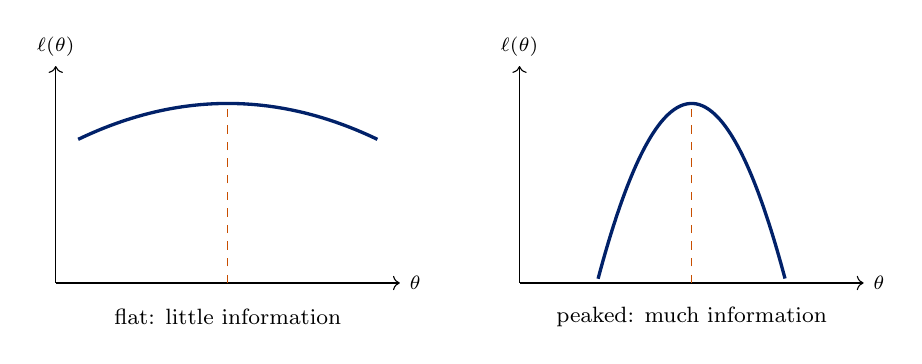
\begin{tikzpicture}[scale=0.95]
  \begin{scope}
    \draw[->] (0,0) -- (4.6,0) node[right]{\scriptsize $\theta$};
    \draw[->] (0,0) -- (0,2.9) node[above]{\scriptsize $\loglik(\theta)$};
    \draw[dukeblue,very thick,smooth,samples=60,domain=0.3:4.3,variable=\x]
      plot ({\x},{2.4-0.12*(\x-2.3)^2});
    \draw[accent,dashed] (2.3,0) -- (2.3,2.4);
    \node at (2.3,-0.45) {\footnotesize flat: little information};
  \end{scope}
  \begin{scope}[xshift=6.2cm]
    \draw[->] (0,0) -- (4.6,0) node[right]{\scriptsize $\theta$};
    \draw[->] (0,0) -- (0,2.9) node[above]{\scriptsize $\loglik(\theta)$};
    \draw[dukeblue,very thick,smooth,samples=60,domain=1.05:3.55,variable=\x]
      plot ({\x},{2.4-1.5*(\x-2.3)^2});
    \draw[accent,dashed] (2.3,0) -- (2.3,2.4);
    \node at (2.3,-0.45) {\footnotesize peaked: much information};
  \end{scope}
\end{tikzpicture}
\end{center}
\vskip2pt
Both log-likelihoods peak at the same $\hat\theta$. But on the left, many nearby
values of $\theta$ fit almost as well; we are uncertain. On the right, moving
away from $\hat\theta$ costs a lot of fit; we are confident.
\vskip3pt
\alert{The second derivative measures exactly this: the more negative, the
more information.}
\end{frame}

\begin{frame}{Fisher Information\core}
\begin{block}{Definition (one parameter, at the true value)}
\begin{align*}
  \Info(\theta_0) \;\equiv\; -\E\!\left[\loglik''(\theta_0)\right]
  \;=\; \E\!\left[S(\theta_0)^{2}\right]
  \;=\; \Var\big(S(\theta_0)\big) .
\end{align*}
\end{block}
\vskip2pt
\textbf{Mind the direction}: the true $\theta_0$ is fixed and the data
vary, Week 2's sampling-distribution view, which is how any estimator is
judged (estimation ran the other way). $\E$ and $\Var$ average over
$y \sim f(y\mid\theta_0)$. Minus sign because $\loglik''<0$ at a peak.
\vskip1pt
\begin{itemize}\itemsep2pt
  \item The second and third forms are the \alert{information equality},
        $-\E[\loglik''] = \Var(S)$: proved in the orange frames, true if the
        model is right. It lets one number, the curvature at the peak, give
        the standard error.
  \item \emph{Additive}: $\loglik$ is a sum of $n$ like terms, so
        $-\E[\loglik'']$ is too: $\Info_n = n\,\Info_1$, the familiar $1/n$.
  \item \textbf{From data}: plug $\hat\theta$ into your sample's own
        $-\loglik''(\theta)$. This is the \emph{observed information},
        what software reports.
\end{itemize}
\end{frame}

\begin{frame}{The Variance of the MLE\core}
\begin{align*}
  \boxed{\;\hat{V}(\hat\theta)
  = \left[-\frac{\partial^2\loglik}{\partial\theta^2}\bigg|_{\hat\theta}\right]^{-1}
  = \frac{1}{\text{observed information}}\;}
\end{align*}
Read it as a sentence: \emph{the variance is one over minus the second
derivative of the log-likelihood at its peak}. \textbf{Why}, in one Newton
step from the truth: the score is zero at the peak, so
\begingroup\setlength{\abovedisplayskip}{2pt}\setlength{\belowdisplayskip}{2pt}
\begin{align*}
  0 = S(\hat\theta) \approx S(\theta_0) + \loglik''(\theta_0)(\hat\theta-\theta_0)
  \ \Longrightarrow\
  \hat\theta - \theta_0 \approx \frac{S(\theta_0)}{-\loglik''(\theta_0)} .
\end{align*}
\endgroup
The score varies across samples with variance $\Info$ (the information
equality); dividing by the curvature $\Info$ leaves
$\Var(\hat\theta) \approx \Info/\Info^2 = 1/\Info$. The orange frames fill
in the steps. This is why \texttt{optim(..., hessian = TRUE)} is not
optional.
\vskip1pt
{\footnotesize Several parameters\adv: the observed information is a matrix
(the Hessian, sign flipped); invert it, and the standard errors are the
square roots of its diagonal.}
\end{frame}

\begin{frame}{Information Equality: Why Care\adv}
The Variance frame's Newton step:
$\hat\theta - \theta_0 \approx S(\theta_0)/(-\loglik''(\theta_0))$. The
denominator is a sum over observations, so by the law of large numbers (as
in Week 2) replace it by its expectation, a fixed number
$1/c = -\E[\loglik''(\theta_0)]$. Then $\Var(cS) = c^2\Var(S)$:
\begin{align*}
  \Var(\hat\theta) \approx
  \frac{\Var\big(S(\theta_0)\big)}{\big(-\E[\loglik''(\theta_0)]\big)^{2}} .
\end{align*}
These are two different quantities. The information equality,
$\Var(S(\theta_0)) = -\E[\loglik''(\theta_0)] = \Info(\theta_0)$, says they
are the same number, so the ratio collapses to $\Info/\Info^2 = 1/\Info$.
\vskip2pt
\begin{itemize}\itemsep2pt
  \item One number, the curvature at the peak, is the whole standard error.
        Without the equality you would need both pieces separately: Week
        2's sandwich.
  \item The $\approx$ is a first-order expansion, exact in the $\sqrt n$
        limit (Properties section).
\end{itemize}
\end{frame}

\begin{frame}{Information Equality: Goal and Plan\adv}
\textbf{What we want to show.} Setting, in three lines: one observation
$y \sim f(y\mid\theta)$; its own score $s(y;\theta) \equiv
\partial\log f(y\mid\theta)/\partial\theta = (\partial f/\partial\theta)/f$,
evaluated at that same true $\theta$; only $y$ is random, and $\E$ averages
over it. The full score is $S = \sum_i s(y_i;\theta)$. Then:
\begingroup
\setlength{\abovedisplayskip}{3pt}\setlength{\belowdisplayskip}{3pt}
\begin{align*}
  -\E\!\left[\frac{\partial^2 \log f}{\partial\theta^2}\right]
  \;=\; \E\big[s^2\big] \;=\; \Var(s) .
\end{align*}
\endgroup
\textbf{The only tool.} The density integrates to one at \emph{every}
$\theta$, so all its $\theta$-derivatives vanish (we may swap $d/d\theta$
and $\int$, one of the ``regularity conditions''):
\begin{align*}
  \int f(y\mid\theta)\,dy = 1 \ \text{ for all }\theta
  \qquad\Longrightarrow\qquad
  \frac{d}{d\theta}\int f(y\mid\theta)\,dy = 0 .
\end{align*}
\textbf{Plan.}
\vskip-2pt
\begin{enumerate}\itemsep0pt
  \item Differentiate once $\Rightarrow$ $\E[s] = 0$.
  \item Differentiate twice $\Rightarrow$ $\E\big[(\partial^2 f/\partial\theta^2)/f\big] = 0$.
  \item Quotient rule on $s$ $\Rightarrow$ $\partial^2\log f/\partial\theta^2 = (\partial^2 f/\partial\theta^2)/f - s^2$.
  \item Take expectations of step 3; steps 1--2 leave only $s^2$.
\end{enumerate}
\end{frame}

\begin{frame}{Information Equality: Steps 1--2\adv}
\textbf{Step 1: differentiate once.}
\begingroup
\setlength{\abovedisplayskip}{2pt}\setlength{\belowdisplayskip}{2pt}
\begin{align*}
  0 &= \frac{d}{d\theta}\int f(y\mid\theta)\,dy
    && \text{\footnotesize derivative of the constant $1$} \\
    &= \int \frac{\partial f(y\mid\theta)}{\partial\theta}\,dy
    && \text{\footnotesize move the derivative inside the integral} \\
    &= \int s(y;\theta)\, f(y\mid\theta)\,dy
    && \text{\footnotesize $s = (\partial f/\partial\theta)/f$, so $\partial f/\partial\theta = s\,f$; $s$ depends on $y$ too} \\
    &= \E\big[s(y;\theta)\big]
    && \text{\footnotesize $\int g(y)\,f(y\mid\theta)\,dy = \E[g(y)]$ for $y\sim f(\cdot\mid\theta)$, this same $\theta$}
\end{align*}
\endgroup
\textbf{Step 2: differentiate twice.} Line two above is $0$ at every $\theta$; differentiate it again:
\begingroup
\setlength{\abovedisplayskip}{2pt}\setlength{\belowdisplayskip}{2pt}
\begin{align*}
  0 &= \int \frac{\partial^2 f(y\mid\theta)}{\partial\theta^2}\,dy
    && \text{\footnotesize derivative of a zero is zero} \\
    &= \int \frac{\partial^2 f/\partial\theta^2}{f}\; f\,dy
     = \E\!\left[\frac{\partial^2 f/\partial\theta^2}{f}\right]
    && \text{\footnotesize multiply and divide by $f$: an expectation}
\end{align*}
\endgroup
\end{frame}

\begin{frame}{Information Equality: Step 3\adv}
\textbf{Step 3: differentiate the score.} $s = (\partial f/\partial\theta)/f$
is a ratio, so use the quotient rule $(u/v)' = (u'v - uv')/v^2$ with
$u = \partial f/\partial\theta$ and $v = f$:
\begingroup
\setlength{\abovedisplayskip}{2pt}\setlength{\belowdisplayskip}{2pt}
\begin{align*}
  \frac{\partial^2 \log f}{\partial\theta^2}
  &= \frac{\partial s}{\partial\theta}
    && \text{\footnotesize $s$ is the first derivative of $\log f$} \\[2pt]
  &= \frac{\dfrac{\partial^2 f}{\partial\theta^2}\, f
          \;-\; \dfrac{\partial f}{\partial\theta}\,\dfrac{\partial f}{\partial\theta}}{f^{2}}
    && \text{\footnotesize $u' = \partial^2 f/\partial\theta^2$, $v' = \partial f/\partial\theta$} \\[2pt]
  &= \frac{\partial^2 f/\partial\theta^2}{f}
     \;-\; \left(\frac{\partial f/\partial\theta}{f}\right)^{\!2}
    && \text{\footnotesize split the fraction; cancel one $f$ in each piece} \\[2pt]
  &= \frac{\partial^2 f/\partial\theta^2}{f} \;-\; s^{2}
    && \text{\footnotesize the bracket is $s$ by definition}
\end{align*}
\endgroup
\vskip2pt
An identity in $y$ and $\theta$, no expectation yet. The first term is the
quantity step 2 showed has mean zero; the second is the squared score.
\end{frame}

\begin{frame}{Information Equality: Step 4\adv}
\textbf{Step 4: take expectations of step 3.}
\begin{align*}
  \E\!\left[\frac{\partial^2 \log f}{\partial\theta^2}\right]
  &= \E\!\left[\frac{\partial^2 f/\partial\theta^2}{f}\right] - \E[s^2]
    && \text{\footnotesize expectation of a difference} \\[3pt]
  &= 0 - \E[s^2]
    && \text{\footnotesize step 2 kills the first term} \\[3pt]
  &= -\Var(s)
    && \text{\footnotesize step 1: $\E[s]=0$, so $\Var(s) = \E[s^2] - 0^2$}
\end{align*}
Multiply by $-1$:
$\;-\E\big[\partial^2 \log f/\partial\theta^2\big] = \Var(s)$. Done, for one observation.
\vskip4pt
\begin{itemize}\itemsep2pt
  \item With $n$ independent observations, $\loglik'' = \sum_i \partial^2\log f(y_i\mid\theta)/\partial\theta^2$
        and $S = \sum_i s(y_i;\theta)$: expectations add, and variances of
        independent terms add, so $-\E[\loglik''] = \Var(S)$ as well.
  \item Every expectation was taken under the \emph{same} $f$ that
        integrates to one. If the data come from some other $g$, steps 1
        and 2 fail, the two sides part ways, and the Hessian standard error
        is wrong.
\end{itemize}
\end{frame}

\begin{frame}{Worked: Bernoulli Information}
\begin{align*}
  S(\theta) &= \frac{\sum_i y_i}{\theta} - \frac{n-\sum_i y_i}{1-\theta}, \\[3pt]
  \frac{\partial^2\loglik}{\partial\theta^2}
  &= -\frac{\sum_i y_i}{\theta^2} - \frac{n - \sum_i y_i}{(1-\theta)^2} .
\end{align*}
Taking expectations, using $\E[\sum_i y_i] = n\theta$:
\begin{align*}
  \Info(\theta)
  = \frac{n\theta}{\theta^2} + \frac{n(1-\theta)}{(1-\theta)^2}
  = \frac{n}{\theta} + \frac{n}{1-\theta}
  = \frac{n}{\theta(1-\theta)} .
\end{align*}
\pause
\begin{align*}
  \Var(\hat\theta) = \Info(\theta)^{-1} = \frac{\theta(1-\theta)}{n} . \quad\checkmark
\end{align*}
Exactly the variance of a sample proportion you already know, now \emph{derived}
from the shape of the likelihood.
\end{frame}

\begin{frame}{Worked: Poisson Information}
\begin{align*}
  \frac{\partial^2\loglik}{\partial\theta^2} = -\frac{\sum_i y_i}{\theta^2}
  \quad\Longrightarrow\quad
  \Info(\theta) = \frac{\E[\sum_i y_i]}{\theta^2} = \frac{n\theta}{\theta^2}
  = \frac{n}{\theta} ,
\end{align*}
so
\begin{align*}
  \Var(\hat\theta) = \frac{\theta}{n},
  \qquad
  \hat{V}(\hat\theta) = \frac{\bar y}{n} .
\end{align*}
\vskip4pt
Check directly: $\hat\theta = \bar y$ and $\Var(\bar Y) = \Var(Y)/n =
\theta/n$, because the Poisson mean equals its variance. \checkmark\ Two
routes, same answer; when a direct calculation exists, use it as a check.
\end{frame}

%%%%%%%%%%%%%%%%%%%%%%%%%%%%%%%%%%%%%%%%%%%%%%%%%%%%%%%%%%%%%%%%%%%%%%%%%%%%%%%
\section[Properties]{Properties of the MLE}
%%%%%%%%%%%%%%%%%%%%%%%%%%%%%%%%%%%%%%%%%%%%%%%%%%%%%%%%%%%%%%%%%%%%%%%%%%%%%%%
\begin{frame}\sectionpage\end{frame}

\begin{frame}{The Four Properties}
Under regularity conditions, as $n\to\infty$:
\begin{enumerate}\itemsep5pt
  \item \textbf{Consistency}\core: $\hat\theta \pto \theta_0$.
  \item \textbf{Asymptotic normality}\core:
        $\hat\theta \overset{a}{\sim} \mathcal N\big(\theta_0, \Info(\theta_0)^{-1}\big)$.
  \item \textbf{Asymptotic efficiency}\adv: if the model is right, no
        other well-behaved estimator has a smaller asymptotic variance (the
        \alert{Cramér--Rao bound}). Stronger than Gauss--Markov, which ranked
        only \emph{linear} unbiased estimators.
  \item \textbf{Invariance}\adv: if $\hat\theta$ is the MLE of $\theta$, then
        $c(\hat\theta)$ is the MLE of $c(\theta)$ for any function $c(\cdot)$.
        Wonderfully convenient: the MLE of the odds is the odds of the MLE.
\end{enumerate}
\vskip6pt
\alert{The first three are asymptotic}, none of them says anything about
$n = 40$. Invariance, by contrast, holds exactly in any sample.
\vskip2pt
{\footnotesize Why 1--2 hold: the Newton step from the truth (Variance
frame), $\hat\theta - \theta_0 \approx S(\theta_0)/(-\loglik''(\theta_0))$,
has a sum in the numerator (CLT: normal) and a sum in the denominator (LLN:
converges to $\Info$), structurally Week 2's OLS argument\adv.}
\end{frame}

\begin{frame}{Maximum Likelihood Is Not Unbiased\core}
\begin{itemize}\itemsep4pt
  \item We already saw it: $\hat\sigma^2_{\text{MLE}} = \frac1n\sum_i \hat e_i^{\,2}$
        has $\E[\hat\sigma^2] = \frac{n-2}{n}\sigma^2$ in the bivariate
        model; $s^2$ divides by $n-2$ precisely to undo this.
\end{itemize}
\vskip6pt
\textbf{The general claim.} Maximum likelihood makes no promise about
unbiasedness in a finite sample. Some MLEs happen to be unbiased (the Poisson
$\hat\theta = \bar y$; $\hat\beta$ in the normal linear model, which is OLS);
others are biased ($\hat\sigma^2$ above). What the method guarantees is that
$\hat\theta$ closes in on $\theta_0$ as $n$ grows (consistency); whatever
bias there is at $n = 40$ is a finite-sample matter that vanishes with it.
\vskip8pt
\begin{alertblock}{The trade we are making}
Give up exact unbiasedness in finite samples; get consistency, asymptotic
efficiency, and a completely general recipe that works for any probability model
you can write down.
\end{alertblock}
\end{frame}

\section[Testing]{Likelihood-Based Tests}

%%%%%%%%%%%%%%%%%%%%%%%%%%%%%%%%%%%%%%%%%%%%%%%%%%%%%%%%%%%%%%%%%%%%%%%%%%%%%%%

\begin{frame}\sectionpage\end{frame}

\begin{frame}{Goal and Plan}
\textbf{What we want.} A test of a hypothesis about $\theta$ that uses
nothing but the log-likelihood curve, and a clear reading of which test
\texttt{R} ran when it printed a $p$-value.
\vskip4pt
\textbf{The plan.}
\begin{enumerate}\itemsep3pt
  \item A null hypothesis is one value, $\theta_0$. The question: is
        $\theta_0$ far from the peak $\hat\theta$?
  \item The obvious ruler, $z = (\hat\theta - \theta_0)/\SE$, works at large
        $n$ and breaks at small $n$ near a boundary.
  \item The curve offers two ways to measure ``far'': the horizontal gap
        (Wald) and the vertical drop in fit (likelihood ratio). On a
        parabola (i.e., with large $n$) they are one number.
  \item Off a parabola they differ. Compute both on Simulation 2's
        samples: which one still works at small $n$?
  \item Which test your software ran, and what to report in practice.
\end{enumerate}
\end{frame}

\begin{frame}{A Null Hypothesis Is a Smaller Model\core}
Week 2 tested $\beta_j = 0$. Look closely at what that null is.
\begin{itemize}\itemsep5pt
  \item $\beta_j = 0$ is the model \emph{without} $X_j$: the same regression
        with one parameter pinned at a fixed value.
  \item In general, $\theta = \theta_0$ is the model with $\theta$ pinned at
        $\theta_0$, the \textbf{restricted} model. The model where $\theta$ is
        free is the \textbf{unrestricted} one; its best value is $\hat\theta$.
\end{itemize}
\vskip6pt
So these are the same question:
\begin{itemize}\itemsep4pt
  \item Is $\hat\beta_j$ statistically significant?
  \item Does the model with $X_j$ fit better than the model without it?
\end{itemize}
\vskip6pt
\begin{center}
\alert{Is the null value $\theta_0$ far from the peak $\hat\theta$?}
\end{center}
One question. The log-likelihood curve will give three ways to measure
``far.'' Start with the one you already know.
\end{frame}

\begin{frame}{The Obvious Ruler: $z$\core}
The last section gave $\hat\theta$ and
$\SE(\hat\theta) = 1/\sqrt{\text{observed information}}$. Week 2's test
divided an estimate by its standard error, so:
\begin{align*}
  z = \frac{\hat\theta - \theta_0}{\SE(\hat\theta)} ,
  \qquad \text{reject if } |z| > 1.96 .
\end{align*}
\begin{itemize}\itemsep5pt
  \item This is the \textbf{Wald test}. It is what \texttt{summary(glm)}
        prints next to every coefficient.
\end{itemize}
\vskip6pt
Does it work? Check it the way Week 2 checked everything: simulate under the
null and count rejections. Two settings, one comfortable, one not.
\end{frame}

\begin{frame}{Simulation 1: $z$ at Large $n$\core}
Poisson counts, true $\theta_0 = 2$, $n = 200$. Draw $20{,}000$ samples;
in each, compute $\hat\theta = \bar y$, $\SE = \sqrt{\hat\theta/n}$ (Worked:
Poisson Information), and $z = (\hat\theta - \theta_0)/\SE$.
\begin{columns}[c]
\begin{column}{0.52\textwidth}
\centering
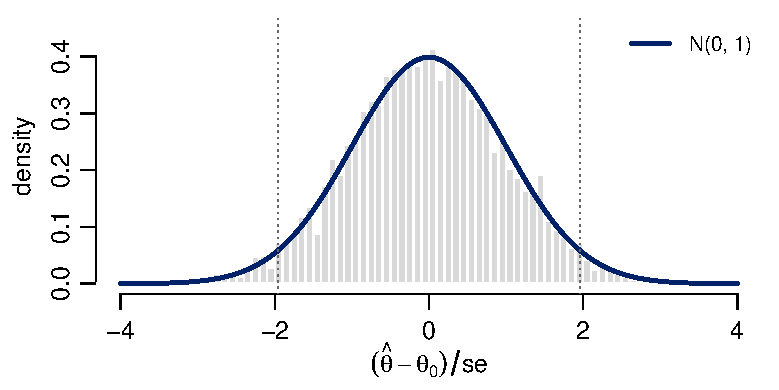
\includegraphics[width=\linewidth]{figs/sim_z_large.pdf}
\end{column}
\begin{column}{0.46\textwidth}
\begin{itemize}\itemsep5pt
  \item The histogram sits on the $\mathcal N(0,1)$ curve.
  \item Reject when $|z| > 1.96$: $5.1\%$ of samples, as advertised.
\end{itemize}
\vskip4pt
\textbf{Verdict}: at large $n$ the ruler works. The normal limit from the
Properties section is doing exactly what it promised.
\end{column}
\end{columns}
\vskip4pt
Before the uncomfortable setting, one change of units that the other
ruler will need.
\end{frame}

\begin{frame}{Square It: $z^2$ and the $\chi^2$}
\begin{columns}[c]
\begin{column}{0.42\textwidth}
\centering
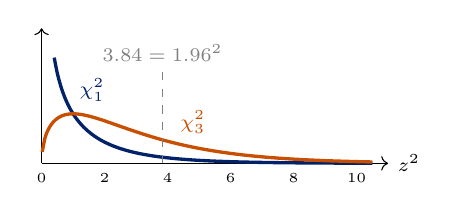
\begin{tikzpicture}[x=0.40cm,y=2.6cm]
  \draw[->] (0,0) -- (11,0) node[right]{\scriptsize $z^2$};
  \draw[->] (0,0) -- (0,0.66);
  % chi2_1 density: exp(-x/2)/sqrt(2 pi x)
  \draw[dukeblue,very thick,smooth,samples=120,domain=0.4:10.5,variable=\x]
    plot ({\x},{exp(-\x/2)/sqrt(2*pi*\x)});
  % chi2_3 density: sqrt(x) exp(-x/2)/2.5066
  \draw[accent,very thick,smooth,samples=120,domain=0.02:10.5,variable=\x]
    plot ({\x},{sqrt(\x)*exp(-\x/2)/2.5066});
  \draw[gray,dashed] (3.84,0) -- (3.84,0.45);
  \node[gray,above] at (3.84,0.45) {\scriptsize $3.84 = 1.96^2$};
  \foreach \t in {0,2,4,6,8,10} \node[below] at (\t,0) {\tiny \t};
  \node[dukeblue] at (1.6,0.36) {\scriptsize $\chi^2_1$};
  \node[accent] at (4.8,0.2) {\scriptsize $\chi^2_3$};
\end{tikzpicture}
\end{column}
\begin{column}{0.56\textwidth}
\begin{itemize}\itemsep4pt
  \item $|z| > 1.96$ is the same event as $z^2 > 1.96^2 = 3.84$. Same
        test, written on the square.
  \item Under the null $z$ is standard normal, so $z^2$ has a fixed
        distribution too. Its name is $\chi^2_1$, ``chi-squared with one
        degree of freedom.'' Its 95\% point is $3.84$ by construction.
  \item Squares add. A null that pins $q$ parameters at once gives $q$
        squared $z$'s summed: $\chi^2_q$, mean $q$, cut-offs $3.84$,
        $5.99$, $7.81$ for $q = 1, 2, 3$.
\end{itemize}
\end{column}
\end{columns}
\end{frame}

\begin{frame}{Simulation 2: Small $n$, Near a Boundary\core}
Bernoulli trials, $\theta_0 = 0.1$, $n = 20$,
$\SE = \sqrt{\hat\theta(1-\hat\theta)/n}$ (Worked: Bernoulli). Draw
$20{,}000$ samples; each is $s$ successes out of $20$, so $z$ takes only a
few values.
\begin{columns}[c]
\begin{column}{0.50\textwidth}
\centering
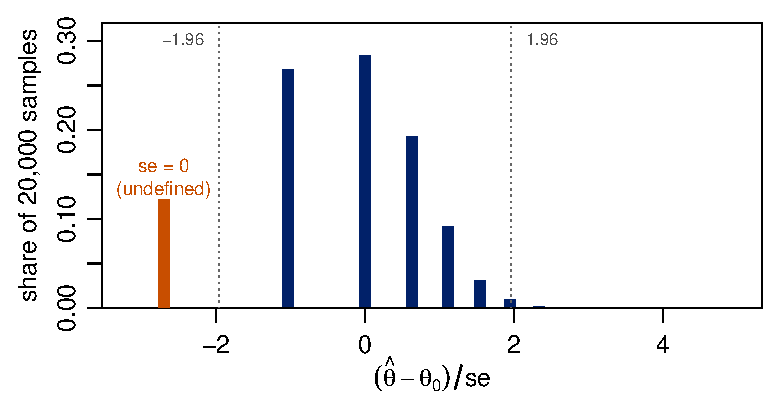
\includegraphics[width=\linewidth]{figs/sim_z_small.pdf}
\end{column}
\begin{column}{0.48\textwidth}
\begin{itemize}\itemsep4pt
  \item $s = 0$ happens in $12\%$ of samples. Then $\hat\theta = 0$,
        $\SE = 0$: $z$ does not exist.
  \item The lowest finite $z$ is $-1.03$ ($s = 1$: $\hat\theta = 0.05$,
        $\SE = 0.049$). The test can \emph{never} reject from below.
  \item It rejects $0.2\%$ of the time, not $5\%$.
\end{itemize}
\vskip4pt
\textbf{Verdict}: the ruler breaks. Why? $z$ uses two numbers, the peak
and its width, and nothing else. What curve is it reading? Take one sample
and draw it.
\end{column}
\end{columns}
\end{frame}

\begin{frame}{Simulation 2: the Curve $z$ Is Reading}
One sample, $s = 2$ of $n = 20$: $\loglik(\theta) = 2\log\theta +
18\log(1-\theta)$, peak $\hat\theta = 0.1$, $\SE =
0.067$ (Worked frames). 

What $z$ ever sees is a peak and a curvature of a parabola 
$\loglik(\hat\theta) - 1/2 \cdot \mathcal{I}\,(\theta-0.1)^2$.
\begin{columns}[c]
\begin{column}{0.56\textwidth}
\centering
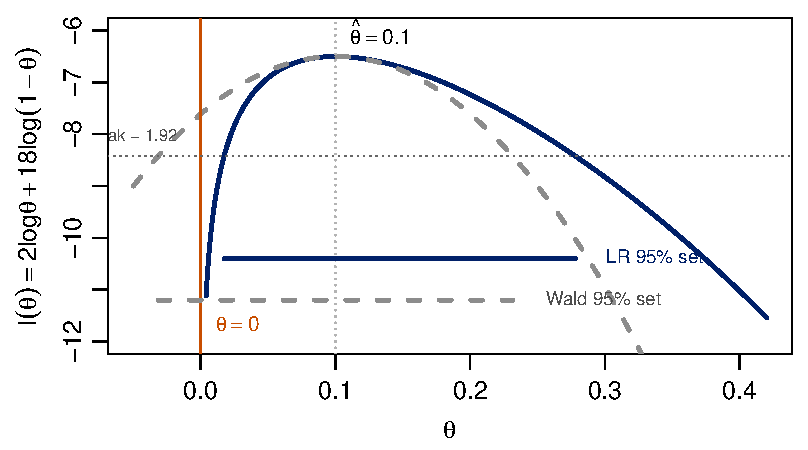
\includegraphics[width=0.88\linewidth]{figs/loglik_n20.pdf}
\end{column}
\begin{column}{0.44\textwidth}
\begin{itemize}\itemsep3pt
  \item Solid: the real $\loglik$. Dashed: the parabola $z$ reads.
  \item \textbf{Left of the peak} the real curve dives to $-\infty$ at
        $\theta = 0$ (two successes are impossible there); the parabola
        sails past into negative probabilities.
\end{itemize}
\end{column}
\end{columns}
\vskip0pt
Wald's 95\% set, $0.1 \pm 1.96 \times 0.067 = (-0.03,\ 0.23)$, contains
impossible values. Is this a small-$n$ disease? Watch the same curve as
$n$ grows.
\end{frame}

\begin{frame}{Large $n$ Makes a Parabola: Watch It Happen}
\begin{columns}[c]
\begin{column}{0.56\textwidth}
\centering
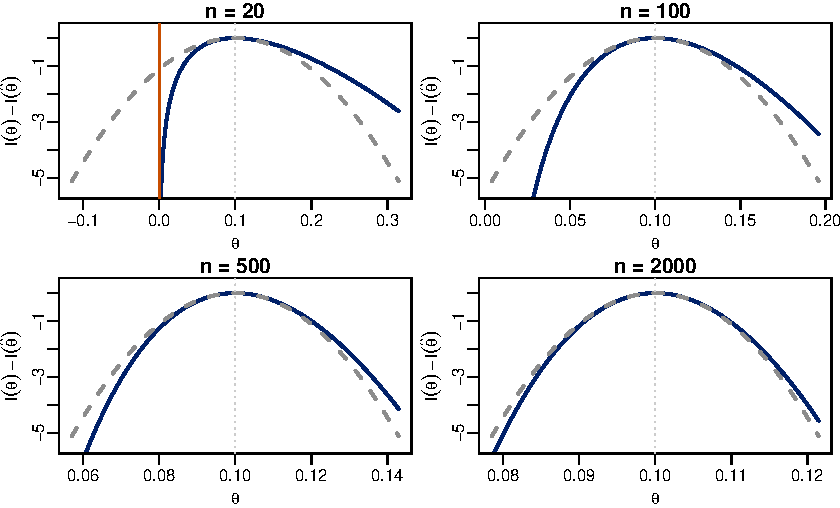
\includegraphics[width=\linewidth]{figs/parabola_n.pdf}
\end{column}
\begin{column}{0.42\textwidth}
Bernoulli with $\hat\theta = 0.1$: the real $\loglik$ (solid) and
the parabola with the same peak and curvature (dashed), each panel
$\hat\theta \pm 3$ SEs.
\vskip8pt
From $n = 20$ to $n = 2000$ the solid curve straightens into the dashed
parabola, exactly over the window a test looks at: a few SEs either side
of the peak. Why? Next frame.
\end{column}
\end{columns}
\end{frame}

\begin{frame}{Why Large $n$ Makes a Parabola\adv}
Expand $\loglik$ around its peak one term past the parabola, and look $c$
standard errors away, at $\theta = \hat\theta + c\,\SE$:
\begingroup
\setlength{\abovedisplayskip}{2pt}\setlength{\belowdisplayskip}{2pt}
\begin{align*}
  \loglik(\hat\theta + c\,\SE) - \loglik(\hat\theta)
  &= -\tfrac12\,\Info\,(c\,\SE)^2 + \tfrac16\,\loglik'''(\hat\theta)\,(c\,\SE)^3 + \cdots
  && \text{\footnotesize Taylor; slope $0$ at the peak} \\
  &= -\frac{c^2}{2} \;+\; \frac{c^3}{6}\cdot\frac{\loglik'''(\hat\theta)}{\Info^{3/2}} + \cdots
  && \text{\footnotesize $\SE = 1/\sqrt{\Info}$}
\end{align*}
\endgroup
\begin{itemize}\itemsep4pt
  \item The first term is the parabola: at $c$ SEs from the peak it drops
        by $c^2/2$, whatever $n$ is.
  \item The second term is the bend away from the parabola. $\loglik$ is a
        sum of $n$ terms, so $\loglik'''$ grows like $n$, while
        $\Info^{3/2}$ grows like $n^{3/2}$: the ratio shrinks like
        $1/\sqrt n$.
\end{itemize}
\vskip4pt
So within a few SEs of the peak, which is the only place a test looks, the
drop is $c^2/2$ plus an error that vanishes as $n$ grows: the last frame's
panels. Next: what exactly a test reads off this curve.
\end{frame}

\begin{frame}{Three Rulers\core}
\begin{center}
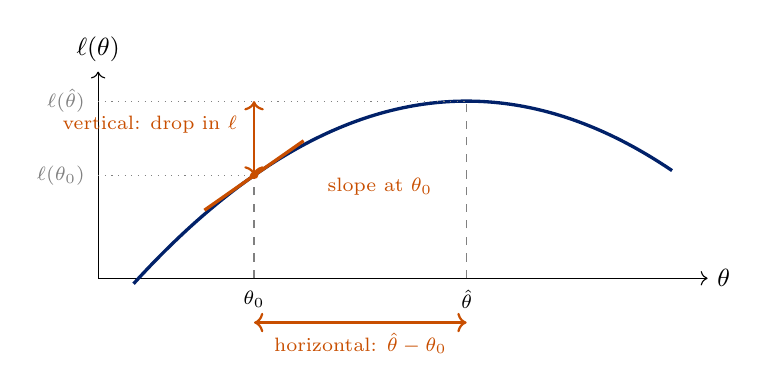
\begin{tikzpicture}[xscale=0.9,yscale=0.75]
  \draw[->] (0,0) -- (8.6,0) node[right]{\small $\theta$};
  \draw[->] (0,0) -- (0,3.5) node[above]{\small $\loglik(\theta)$};
  \draw[dukeblue,very thick,smooth,samples=80,domain=0.5:8.1,variable=\x]
    plot ({\x},{3.0-0.14*(\x-5.2)^2});
  \draw[dashed,gray] (5.2,0) -- (5.2,3.0);
  \node at (5.2,-0.35) {\scriptsize $\hat\theta$};
  \draw[dashed,gray] (2.2,0) -- (2.2,1.74);
  \node at (2.2,-0.35) {\scriptsize $\theta_0$};
  \draw[dotted,gray] (0,3.0) -- (5.2,3.0);
  \draw[dotted,gray] (0,1.74) -- (2.2,1.74);
  \node[gray,anchor=east] at (-0.05,3.0) {\scriptsize $\loglik(\hat\theta)$};
  \node[gray,anchor=east] at (-0.05,1.74) {\scriptsize $\loglik(\theta_0)$};
  \draw[accent,thick,<->] (2.2,1.74) -- (2.2,3.0);
  \node[accent,left] at (2.1,2.6) {\scriptsize vertical: drop in $\loglik$};
  \draw[accent,thick,<->] (2.2,-0.75) -- (5.2,-0.75);
  \node[accent] at (3.7,-1.1) {\scriptsize horizontal: $\hat\theta - \theta_0$};
  \draw[accent,very thick] (1.5,{1.74+0.84*(1.5-2.2)}) -- (2.9,{1.74+0.84*(2.9-2.2)});
  \fill[accent] (2.2,1.74) circle (0.06);
  \node[accent,anchor=west] at (3.1,1.55) {\scriptsize slope at $\theta_0$};
\end{tikzpicture}
\end{center}
\vskip-4pt
\begin{itemize}\itemsep4pt
  \item \textbf{Horizontal}: the gap $\hat\theta - \theta_0$, in
        standard-error units. \hfill \emph{Wald: the $z$-test}
  \item \textbf{Vertical}: the fit lost by moving from $\hat\theta$ down to
        $\theta_0$. \hfill \emph{Likelihood ratio}
  \item \textbf{Slope at $\theta_0$}: at a peak it would be zero. A third
        ruler; we use it in Week 4. \hfill \emph{Score}
\end{itemize}
\end{frame}

\begin{frame}{Two Rulers: the Formulas\core}
Each is a squared $z$, so each is compared with $\chi^2_1$: reject above
$3.84$.
\begin{itemize}\itemsep6pt
  \item \textbf{Wald: the gap over its standard error, squared.}
        $W = z^2 = \Info\,(\hat\theta-\theta_0)^2$, where
        $\Info = -\loglik''(\hat\theta)$ is the observed information and
        $\SE = 1/\sqrt{\Info}$ (Variance frame).
  \item \textbf{Likelihood ratio: the drop in fit, doubled.}
        $LR = 2\,[\loglik(\hat\theta) - \loglik(\theta_0)]$. Never negative,
        because the peak is the highest point. Why doubled: next frame.
\end{itemize}
\vskip4pt
{\footnotesize With $q$ restrictions:
$LR = 2\,[\loglik(\hat\theta_{\text{unrestricted}}) -
\loglik(\hat\theta_{\text{restricted}})] \dto \chi^2_q$, and likewise $W$.
The one-parameter case has $\hat\theta_{\text{restricted}} = \theta_0$.}
\end{frame}

\begin{frame}{On a Parabola, the Two Rulers Are One Number}
Suppose $\loglik$ \emph{is} the parabola with peak $\hat\theta$ and
curvature $-\Info$:
\begingroup
\setlength{\abovedisplayskip}{2pt}\setlength{\belowdisplayskip}{2pt}
\begin{align*}
  \loglik(\theta) &= \loglik(\hat\theta) - \tfrac12\,\Info\,(\theta-\hat\theta)^2
    && \text{\footnotesize the parabola: peak at $\hat\theta$, curvature $-\Info$} \\
  \loglik(\hat\theta) - \loglik(\theta_0) &= \tfrac12\,\Info\,(\hat\theta-\theta_0)^2
    && \text{\footnotesize plug in $\theta = \theta_0$: the drop} \\
  LR = 2 \times \text{drop} &= \Info\,(\hat\theta-\theta_0)^2 = W
    && \text{\footnotesize doubling undoes the $\tfrac12$}
\end{align*}
\endgroup
\begin{itemize}\itemsep2pt
  \item So $W = LR$: one distance, two names, one cut-off.
  \item Read the $LR$ line backwards: $LR > 3.84$ is $\text{drop} > 1.92$,
        Simulation 2's dotted line. ``$1.96$ SEs from the peak'' and
        ``$1.92$ below the peak'' are the same set of $\theta$'s.
\end{itemize}
So the rulers agree exactly when \alert{$\loglik$ is a parabola}.
Simulation 2's curve was not one: compute both on it.
\end{frame}

\begin{frame}{Simulation 2, Continued: Both Rulers}
Same setting, both rulers. Exact rejection rates at $3.84$, true
$\theta_0 = 0.1$:
\vskip-2pt
\begin{center}
\renewcommand{\arraystretch}{1.0}
\begin{tabular}{rccc}
\toprule
$n$ & $W$ undefined & $W$ rejects & $LR$ rejects \\
\midrule
20   & $12.2\%$ & $0.2\%$  & $13.3\%$ \\
50   & $0.5\%$  & $11.6\%$ & $5.8\%$  \\
100  & $0$      & $6.8\%$  & $4.4\%$  \\
500  & $0$      & $5.7\%$  & $5.2\%$  \\
\bottomrule
\end{tabular}
\end{center}
\vskip1pt
\begin{itemize}\itemsep2pt
  \item $n = 20$: neither ruler is at $5\%$. The $s = 0$ samples show why:
        $W$ does not exist, and $LR = 2[0 - 20\log 0.9] = 4.21$ rejects a
        sample that occurs $12\%$ of the time under the null. Two expected
        successes: no parabola; use an exact binomial test.
  \item $n = 50$: $W$'s failure flips. One or two successes give a tiny
        $\SE$, so a huge $|z|$: $W$ rejects $11.6\%$. $LR$ is near $5\%$.
  \item $n \ge 100$: both settle toward $5\%$, $W$ the slower: $LR$
        reads the curve, $W$ extrapolates it. Each row down is the
        parabola arriving, as the panels showed.
\end{itemize}
\end{frame}

\begin{frame}{Which Test Your Software Ran\core}
At large $n$ the two rulers agree. In a small sample or near a boundary
(Simulation 2) they do not, and it matters which one you are reading.
\vskip6pt
\begin{block}{In your output}
\begin{itemize}\itemsep4pt
  \item \texttt{summary(glm)} $z$-statistics and $p$-values: \textbf{Wald}.
  \item \texttt{anova(m0, m1, test = "Chisq")}, the deviance, ``does
        adding this block improve the fit'': \textbf{likelihood ratio}.
\end{itemize}
\end{block}
\vskip6pt
\textbf{When Wald and LR disagree, believe LR}: it measured the curve,
$z$ extrapolated it. The next frame says which one to reach for.
\end{frame}

\begin{frame}{In Practice: What to Report\core}
\begin{block}{The working rules}
\begin{itemize}\itemsep5pt
  \item \textbf{One coefficient, large $n$, an ordinary variable}: the Wald
        $z$ and $p$ that \texttt{summary()} prints are fine. That is what
        published tables report, and at large $n$ it equals LR.
  \item \textbf{A block}: dummies for a categorical variable, an
        interaction, a set of controls, ``does adding these help.'' Fit both
        models and use LR: \texttt{anova(m0, m1, test = "Chisq")}. No
        single $z$ answers that question (Lab 3, region).
  \item \textbf{A rare outcome, a small group, a huge standard error, a
        coefficient near a boundary}: do not trust $z$. Refit without the
        term and report LR.
\end{itemize}
\end{block}
\vskip4pt
The habit to build: when a $z$ looks strange, ask what curve it read.
\end{frame}

\end{document}
